\documentclass{article}
\usepackage{amsmath}
\usepackage{graphicx}
\usepackage{float}

\author{Hossein Kazemi}
\date{}

\begin{document}


\section*{Q1. Loss Function}

\begin{equation}
\mathcal{L} = \mathbb{E}_{x_0,\,t,\,\epsilon} \; \left\| \epsilon - \epsilon_\theta(x_t, t, y) \right\|^2
\end{equation}

where:
\begin{itemize}
    \item $x_0$ is the clean SDF,
    \item $x_t$ is the noisy SDF at timestep $t$,
    \item $\epsilon$ is the Gaussian noise added to $x_0$,
    \item $\epsilon_\theta(\cdot)$ is the model prediction,
    \item $y$ is the conditioning stress--strain curve.
\end{itemize}

Thus, the model learns to predict and remove noise.

\vspace{0.5cm}

\section*{Q2. Loss History}

\begin{figure}[H]
    \centering
    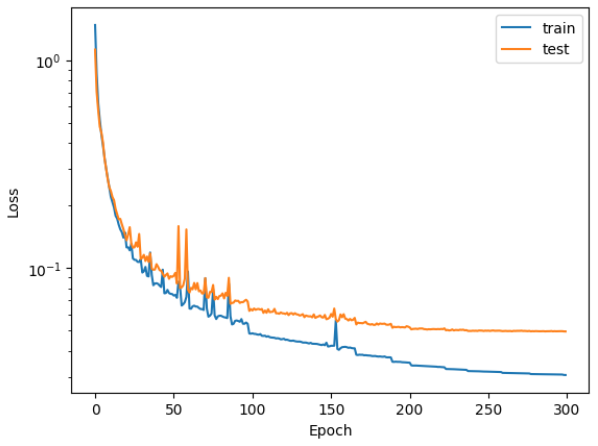
\includegraphics[width=0.7\linewidth]{diffusion_training_history.png}
\end{figure}
The small gap between training and validation loss suggests limited overfitting and good generalization.

\vspace{0.5cm}

\section*{Q3. Biggest Challenge}

The main challenge in the VAR-based approach is that it requires training a VQ-VAE to discretize the continuous SDF space into tokens, which currently results in poor-quality reconstructions and consequently degrades the generated samples (see Fig.~\ref{fig:var_samples}).

\begin{figure}[H]
    \centering
    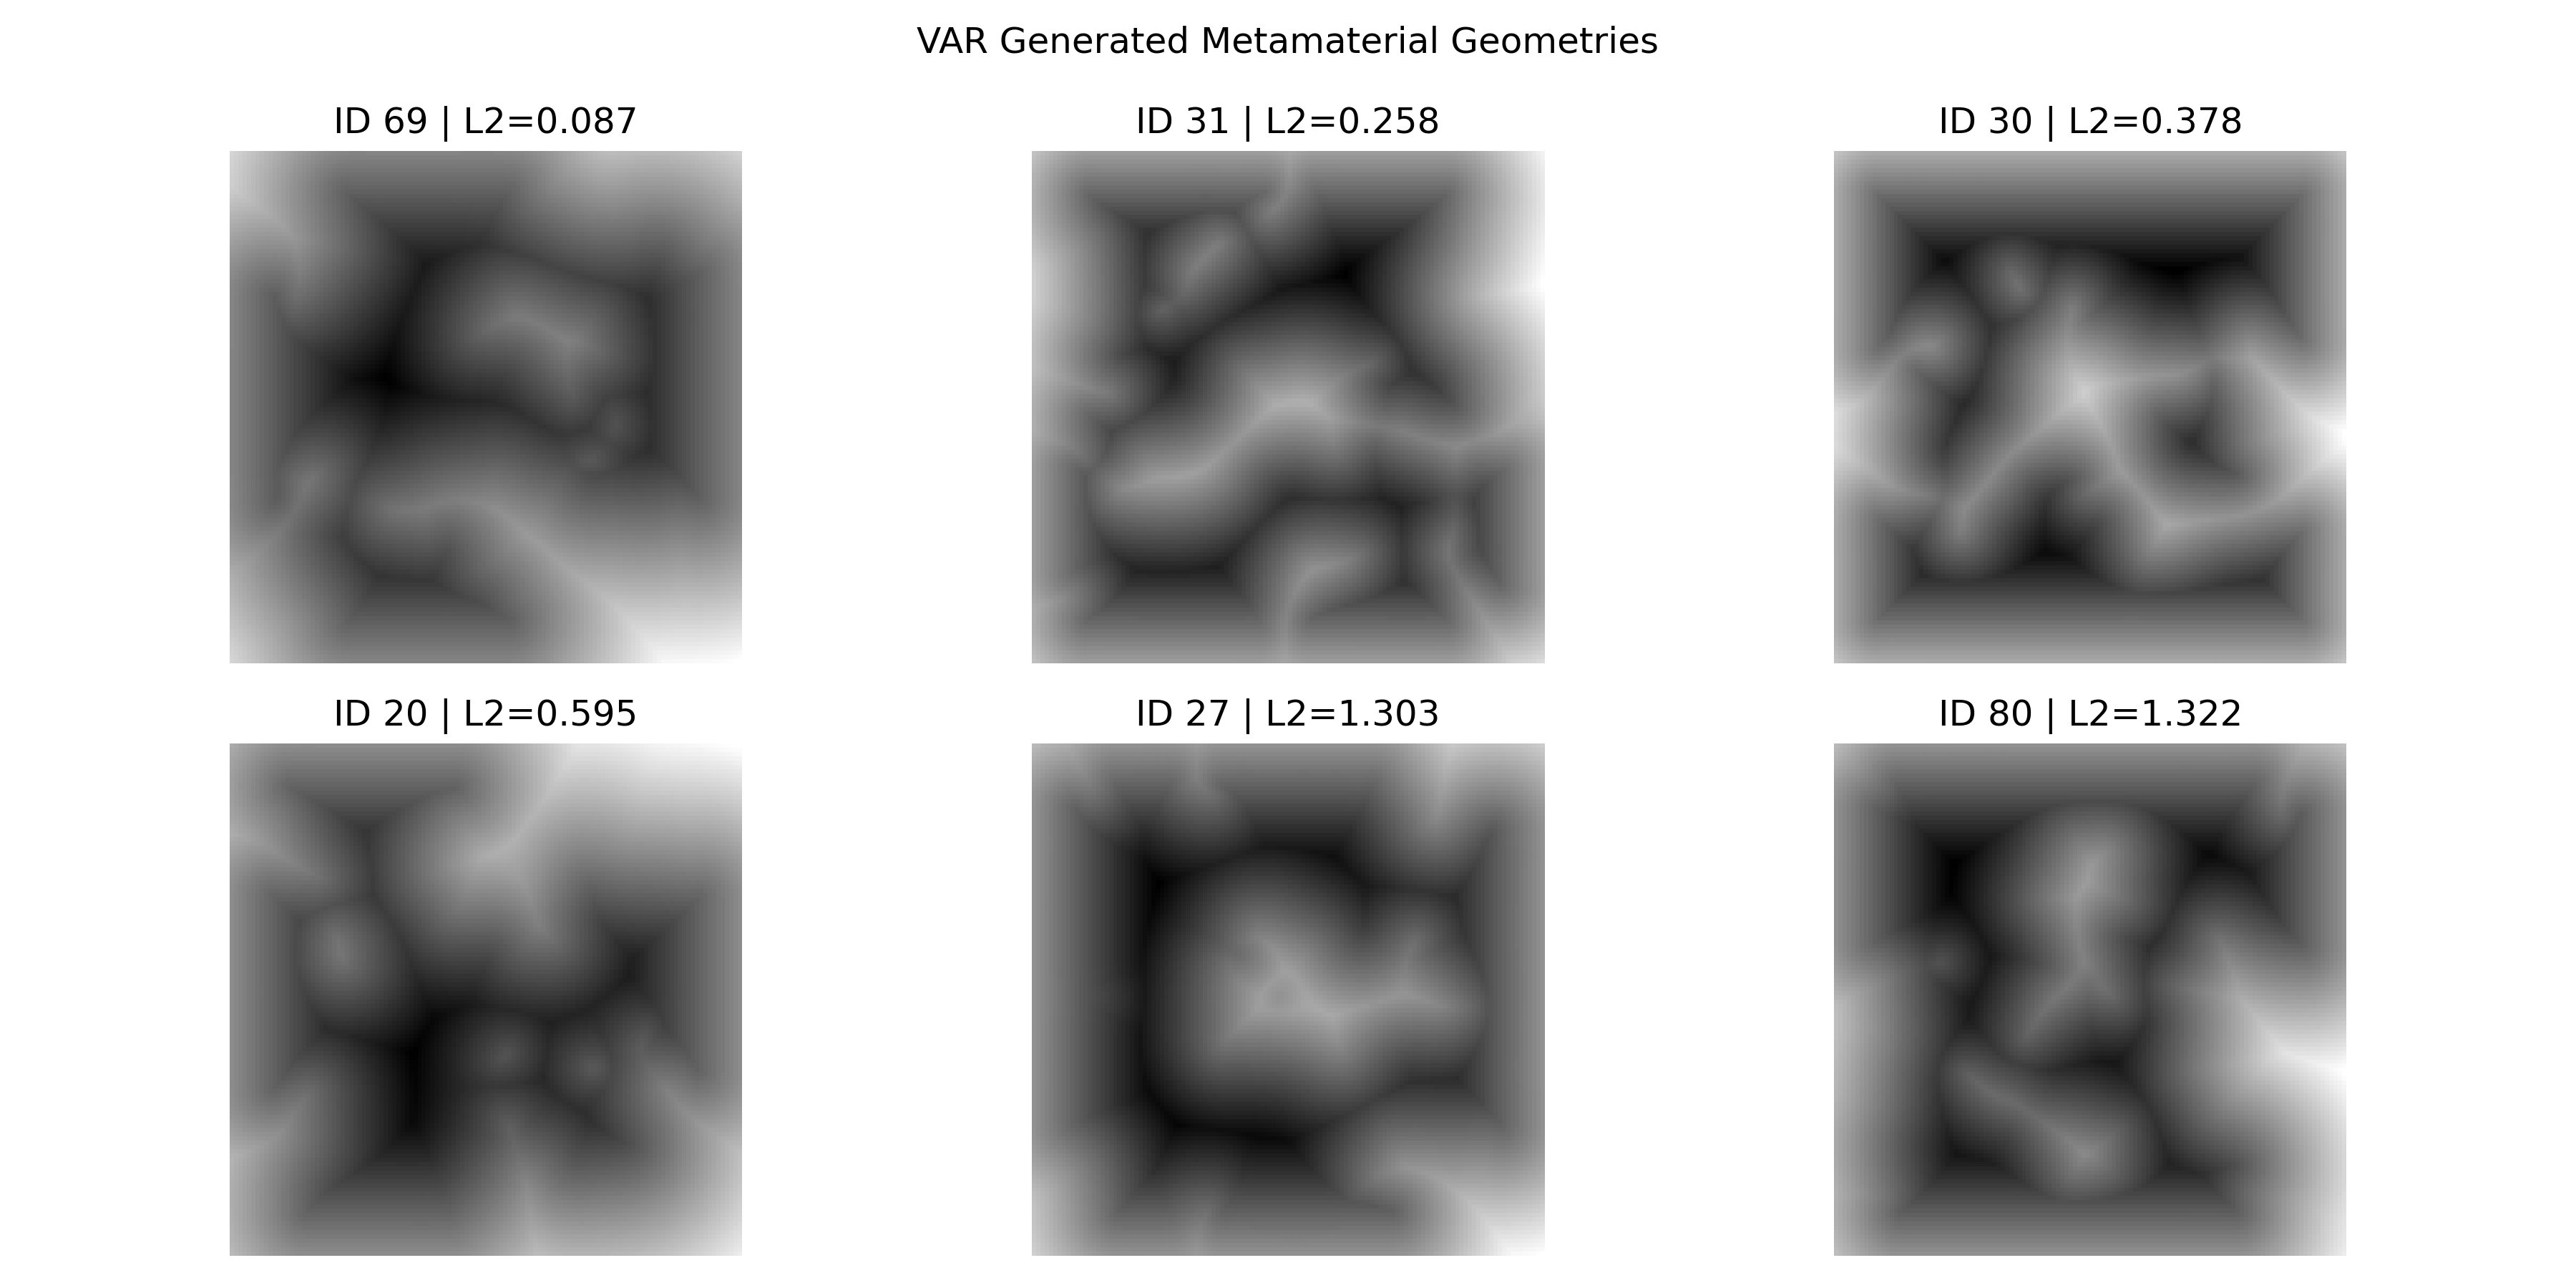
\includegraphics[width=0.8\linewidth]{var_samples_grid.png}
    \label{fig:var_samples}
\end{figure}


The original VAR framework relies on hierarchical resolution prediction, where images are generated progressively from low to high resolution through a multi-scale token generation process, as illustrated in Fig.~\ref{fig:var_framework}.

\begin{figure}[H]
    \centering
    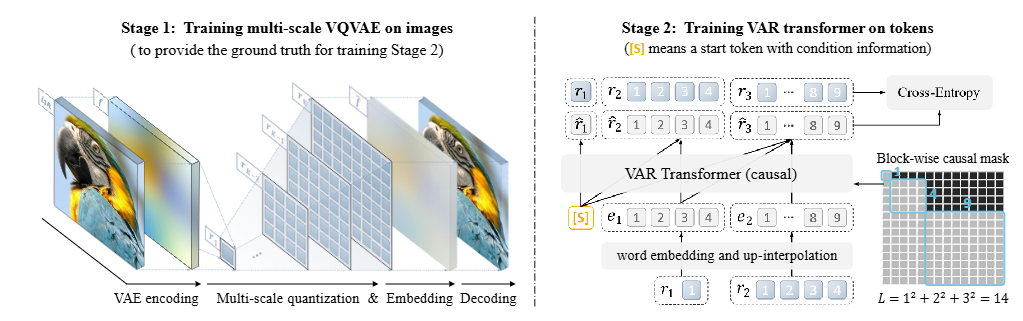
\includegraphics[width=0.9\linewidth]{VAR.png}
    \label{fig:var_framework}
\end{figure}
\end{document}